%%%%%%%%%%%%%%%%%%%%%%%%%%%%%%%%%%%%%%%%%
% baposter Portrait Poster
% LaTeX Template
% Version 1.0 (15/5/13)
%
% Created by:
% Brian Amberg (baposter@brian-amberg.de)
%
% This template has been downloaded from:
% http://www.LaTeXTemplates.com
%
% License:
% CC BY-NC-SA 3.0 (http://creativecommons.org/licenses/by-nc-sa/3.0/)
%
%%%%%%%%%%%%%%%%%%%%%%%%%%%%%%%%%%%%%%%%%

%----------------------------------------------------------------------------------------
%	PACKAGES AND OTHER DOCUMENT CONFIGURATIONS
%----------------------------------------------------------------------------------------

\documentclass[a0paper,portrait]{baposter}

\usepackage[font=footnotesize,labelfont=bf]{caption} % Required for specifying captions to tables and figures
\usepackage{booktabs} % Horizontal rules in tables
\usepackage{relsize} % Used for making text smaller in some places
\usepackage[utf8x]{inputenc}
\usepackage[superscript,biblabel]{cite}


\graphicspath{{figures/}} % Directory in which figures are stored

\definecolor{bordercol}{RGB}{40,40,40} % Border color of content boxes
\definecolor{headercol1}{RGB}{186,215,230} % Background color for the header in the content boxes (left side)
\definecolor{headercol2}{RGB}{80,80,80} % Background color for the header in the content boxes (right side)
\definecolor{headerfontcol}{RGB}{0,0,0} % Text color for the header text in the content boxes
\definecolor{boxcolor}{RGB}{186,215,230} % Background color for the content in the content boxes

\begin{document}

\background{ % Set the background to an image (background.pdf)
\begin{tikzpicture}[remember picture,overlay]
\draw (current page.north west)+(-2em,2em) node[anchor=north west]
{
\includegraphics[height=1.1\textheight]{background.pdf}};
\end{tikzpicture}
}

\begin{poster}{
grid=false,
borderColor=bordercol, % Border color of content boxes
headerColorOne=headercol1, % Background color for the header in the content boxes (left side)
headerColorTwo=headercol2, % Background color for the header in the content boxes (right side)
headerFontColor=headerfontcol, % Text color for the header text in the content boxes
boxColorOne=boxcolor, % Background color for the content in the content boxes
headershape=roundedright, % Specify the rounded corner in the content box headers
headerfont=\Large\sf\bf, % Font modifiers for the text in the content box headers
textborder=rectangle,
background=user,
headerborder=open, % Change to closed for a line under the content box headers
boxshade=plain
}
{}
%
%----------------------------------------------------------------------------------------
%	TITLE AND AUTHOR NAME
%----------------------------------------------------------------------------------------
%
{\sf\bf \huge{ Improving  early epidemiological  assessment of Zika virus epidemics  using historical data}} % Poster title
{ \underline{Julien Riou}, Chiara Poletto, Pierre-Yves Boëlle\\ % Author names
{\smaller \textit{ Sorbonne Universités, Inserm/UPMC, Institut Pierre Louis d’Epidémiologie et de Santé Publique (IPLESP UMRS 1136), Paris, France} \\ 
 \small{[ julien.riou@iplesp.upmc.fr ]}}} % Author email addresses
{
\includegraphics[scale=.25]{logos2.pdf}} % University/lab logo

%----------------------------------------------------------------------------------------
%	INTRODUCTION
%----------------------------------------------------------------------------------------

\headerbox{Introduction}{name=introduction,column=0,row=0}{
\begin{flushleft}
In the early epidemic phase, model-based epidemiological assessment is often conducted to support decision-making by public health authorities.
However, long-term forecast is generally unreliable at this point, as it relies on insufficient information recovered from the few data points available  in real time.\cite{heesterbeek2015modeling}

\hfill \break
We propose to complement this information with \textbf{historical data on similar epidemics}, to be integrated in the analysis under the form of \textbf{informative prior distributions}.
\end{flushleft}
}

%----------------------------------------------------------------------------------------
%	MATERIALS AND METHODS
%----------------------------------------------------------------------------------------

\headerbox{Materials and Methods}{name=methods,column=0,below=introduction}{
\begin{flushleft}
This approach was retrospectively applied to the \textbf{2015-2017 Zika virus epidemics in the French West Indies} (FWI). 
We used a Bayesian dynamic discrete-time SIR model, where the observed incidence $O_t$ depends on
\begin{eqnarray}
O_{t}\sim \mbox{Neg-Bin} \left( R_0 \frac{S_{t}}{N} I^*_t, \phi \right)
\end{eqnarray}

where $R_0$ is the \textbf{basic reproduction number}, $S_t / N$ is the proportion of susceptibles (which depends on past incidence and the \textbf{reporting rate} $\rho$); $I^*_t$ summarizes exposure (past incidence weighted by the discretized serial interval); and $\phi$ is the dispersion parameter.

\hfill \break
This model was implemented in \textit{Stan}.\cite{carpenter2015stan}
It was fitted to increasing amounts of incidence data from Guadeloupe, Martinique and Saint-Martin to obtain posterior distributions for $R_0$ and $\rho$ at different points of the epidemics.
The remaining of the epidemic was then simulated stochastically, leading to a \textbf{predictive distribution of future incidence}.

\hfill \break
Informative priors for $R_0$ and $\rho$ were obtained by combining the results of fitting a two-level \textbf{hierarchical} dynamic SIR model to historical data on earlier CHIKV outbreaks in the FWI (2013-2015) and CHIKV and ZIKV outbreaks French Polynesia (2013-2015), accounting for the similarities and differences between CHIKV and ZIKV transmission and reporting. \cite{riou2017comparative}

\hfill \break
Forecasts were thus conducted using each of three choices of prior distributions:
\begin{itemize}
\itemsep0em
\item \textbf{Non-informative priors} (baseline);
\item \textbf{Regional priors} (island-averaged, from top-level parameters);
\item \textbf{Local priors} (island-specific, from bottom-level parameters).
\end{itemize}


\end{flushleft}
}

%----------------------------------------------------------------------------------------
%	CONCLUSION
%----------------------------------------------------------------------------------------

%\headerbox{Conclusion}{name=conclusion,column=0,below=methods}{
%
%}

%----------------------------------------------------------------------------------------
%	REFERENCES
%----------------------------------------------------------------------------------------

\headerbox{References}{name=references,column=0,below=methods}{

\smaller % Reduce the font size in this block
\renewcommand{\section}[2]{\vskip 0.05em} % Get rid of the default "References" section title
\nocite{*} % Insert publications even if they are not cited in the poster

\bibliographystyle{unsrt}
\bibliography{sample} % Use sample.bib as the bibliography file
}

%----------------------------------------------------------------------------------------
%	ACKNOWLEDGEMENTS
%----------------------------------------------------------------------------------------

%\headerbox{Contact}{name=acknowledgements,column=0,below=references, above=bottom}{
%
%\smaller % Reduce the font size in this block
%Julien Riou, M.D., PhD candidate \\
%julien.riou@iplesp.upmc.fr
%+336 67 50 94 59
%} 

%----------------------------------------------------------------------------------------
%	RESULTS 1
%----------------------------------------------------------------------------------------

\headerbox{Results: eliciting priors from historical data}{name=results1,span=2,column=1,row=0}{ % To reduce this block to 1 column width, remove 'span=2'
The \textbf{regional} informative priors, suitable for a ZIKV outbreak in a typical island of the French West Indies, were relatively wide, with 95\% credible intervals between 0.5 and 2.5 for $R_0$ and between 0 and 0.30 for $\rho$. 
The \textbf{local} informative priors carried specific information from past outbreaks in each island and had a narrower range, especially in Guadeloupe and Martinique.
\begin{center}
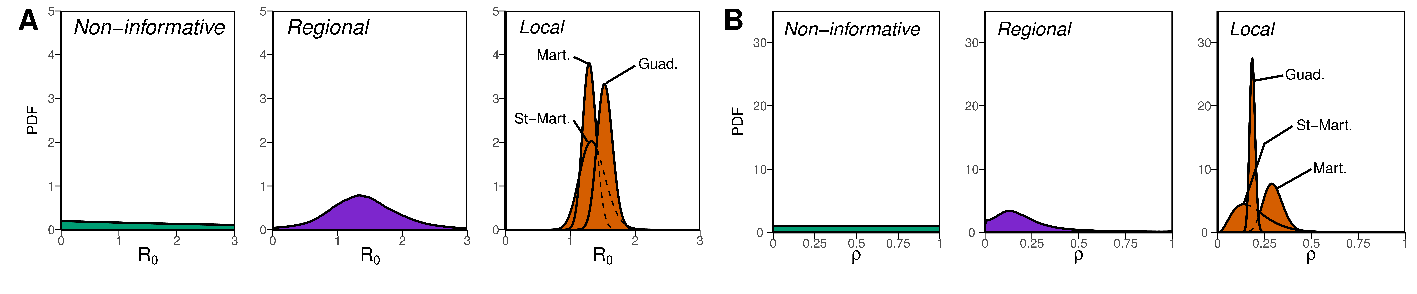
\includegraphics[width=.95\linewidth]{figures/FigPRIOR2.pdf}
\captionof{figure}{{Three choices of prior distributions for the parameters $R_0$ (panel A) and $\rho$ (panel B).}}
\end{center}
}

%----------------------------------------------------------------------------------------
%	RESULTS 2
%----------------------------------------------------------------------------------------

\headerbox{Resutls: epidemic forecast}{name=results2,span=2,column=1,below=results1}{ % To reduce this block to 1 column width, remove 'span=2'

An example of the predictive distribution of future incidence in Martinique is show in Fig. 2A. 
At this point in time, predictions with non-informative priors were largely off-target and showed considerable uncertainty. 
Using informative priors led to major improvements in both \textbf{accuracy }(distance with actual observations) and \textbf{sharpness }(width of the 95\% prediction interval).
These results were typical during the initial phases of the three epidemics.
Once the peak of incidence was reached, the choice of the prior distributions was less critical to prediction quality.
\begin{center}
\includegraphics[width=.95\linewidth]{figures/FigPRED2.pdf}
\captionof{figure}{{(A) Predictive distribution of future incidence in Martinique on January 31st, 2016. (B-C) Accuracy and sharpness of the predictive distribution of incidence according to the date of analysis.}}
\end{center}

%------------------------------------------------

Early forecasts of \textbf{epidemic size} and \textbf{maximal incidence} showed more accuracy and stability when using regional and particularly local priors.
However, forecasts of the date of peak incidence and of the duration of the period of high epidemic activity were less affected by the choice of priors.

\begin{center}
\includegraphics[width=.95\linewidth]{figures/FigINDIC2.pdf}
\captionof{figure}{{Early forecasts regarding four indicators of operational interest: (A) final epidemic size; (B) maximal incidence; (C) date of peak incidence (difference with the eventually observed date in months); and (D) duration of the period of high epidemic activity (in months). Dashed lines represent actual values.}}
\end{center}

}

%----------------------------------------------------------------------------------------


%----------------------------------------------------------------------------------------
%	RESULTS 2
%----------------------------------------------------------------------------------------

\headerbox{Conclusions}{name=conc,span=2,column=1,below=results2,above=bottom}{ % To reduce this block to 1 column width, remove 'span=2'


Our results suggest that during the initial stage of an epidemic, epidemiological forecasting may benefit from using informative priors on key parameters, increasing the accuracy and the stability of the predictions.
If a theoretical framework allows it, these informative priors can be elicited from historical data on previous, similar epidemics using hierarchical models. 
This approach could provide public health authorities with reliable forecasts at an earlier stage than is usually possible.
}

%----------------------------------------------------------------------------------------






\end{poster}

\end{document}